% SPDX-License-Identifier: MIT
% Copyright (c) 2017-2020 Forschungszentrum Juelich GmbH
% This code is licensed under MIT license (see the LICENSE file for details)
%
\documentclass{beamer}
\usetheme{Juelich}
% enable the \fzjset line to allow compat colors globally
% disabled by default since v18.10
\fzjset{compat mode=enabled}
\setlength{\abovecaptionskip}{0pt plus 0pt minus 0pt}

\bibliography{references.bib}
\usepackage{physics}

\title{GPU-Isle}
\author{Marcel, Stefan, Johann, Jan-Lukas}
\institute{JSC, JSC, Uni Bonn, ESS}
\date{\today}
\titlegraphic{\includegraphics%
    [width=\paperwidth]{placeholder}}
\begin{document}
\maketitle

\setbeamertemplate{caption}{\raggedright\insertcaption\par}
\begin{frame}{GPU-Isle Team}
\begin{columns}
\begin{column}{0.25\textwidth}
\begin{figure}

\includegraphics[width=4em,height=6em]{HackathonSlides/Pictures/Marcel_Rodekamp.jpg}
\caption{Marcel Rodekamp}
\end{figure}
\end{column}
\begin{column}{0.25\textwidth}
\begin{figure}
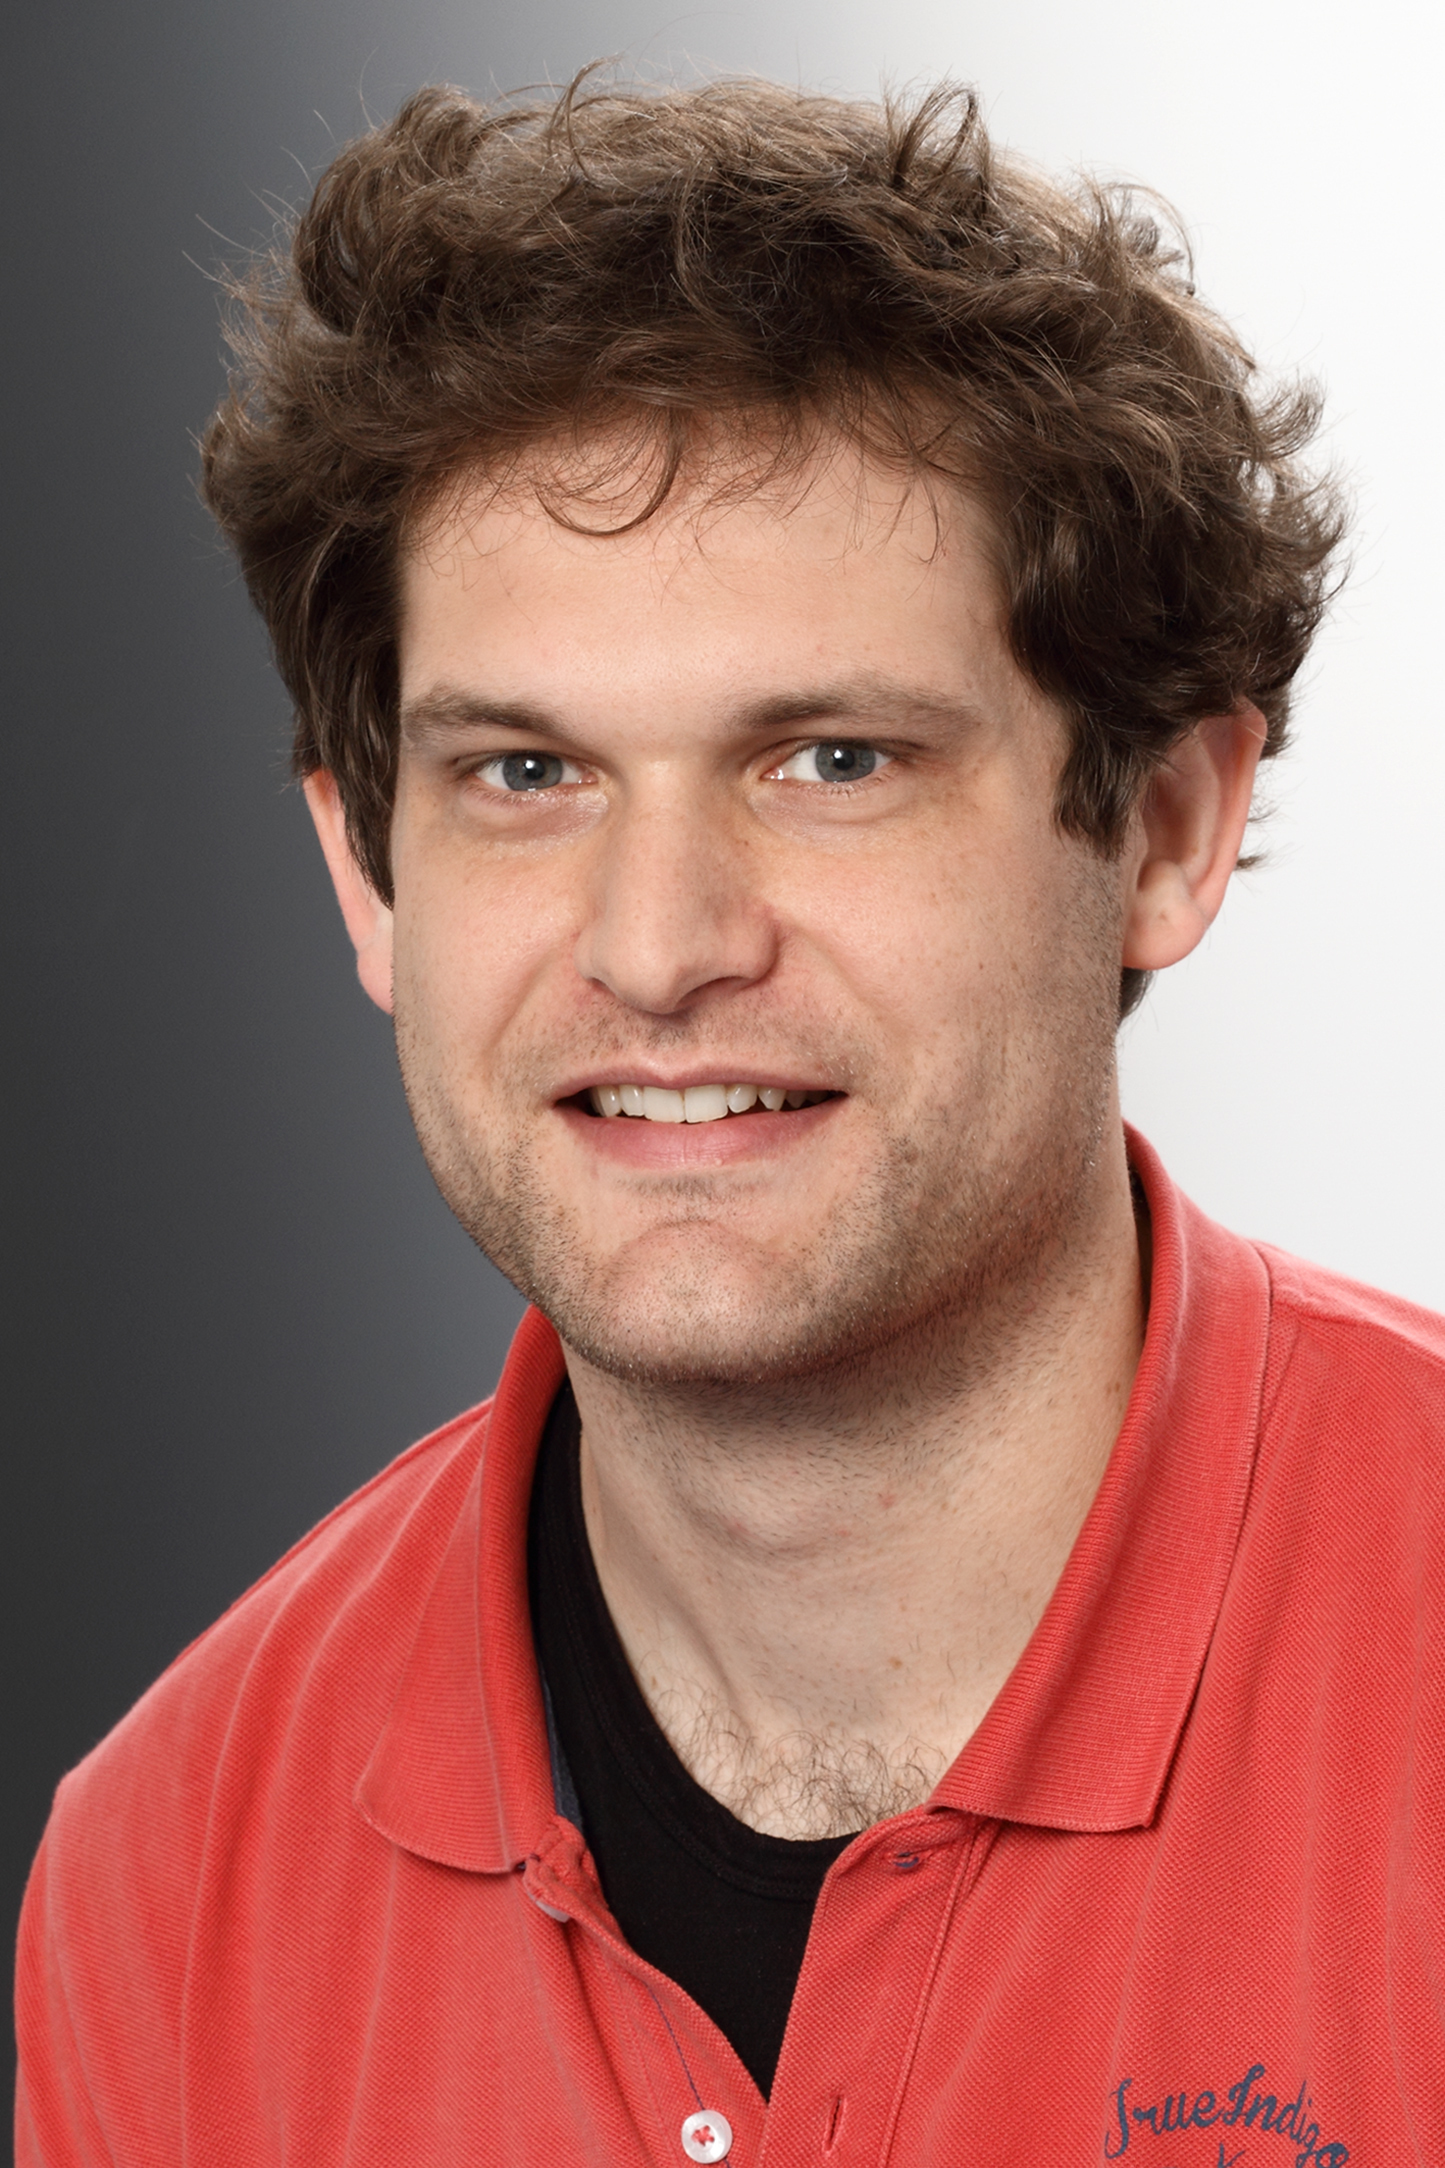
\includegraphics[width=5em,height=6em]{HackathonSlides/Pictures/krieg_009e.jpg}
\caption{Stefan Krieg}
\end{figure}
\end{column}
\begin{column}{0.25\textwidth}
\begin{figure}

\includegraphics[width=5em,height=6em]{HackathonSlides/Pictures/johann_greiser_kopf.jpg}
\caption{Johann Ostmeyer}
\end{figure}
\end{column}
\begin{column}{0.25\textwidth}
\begin{figure}
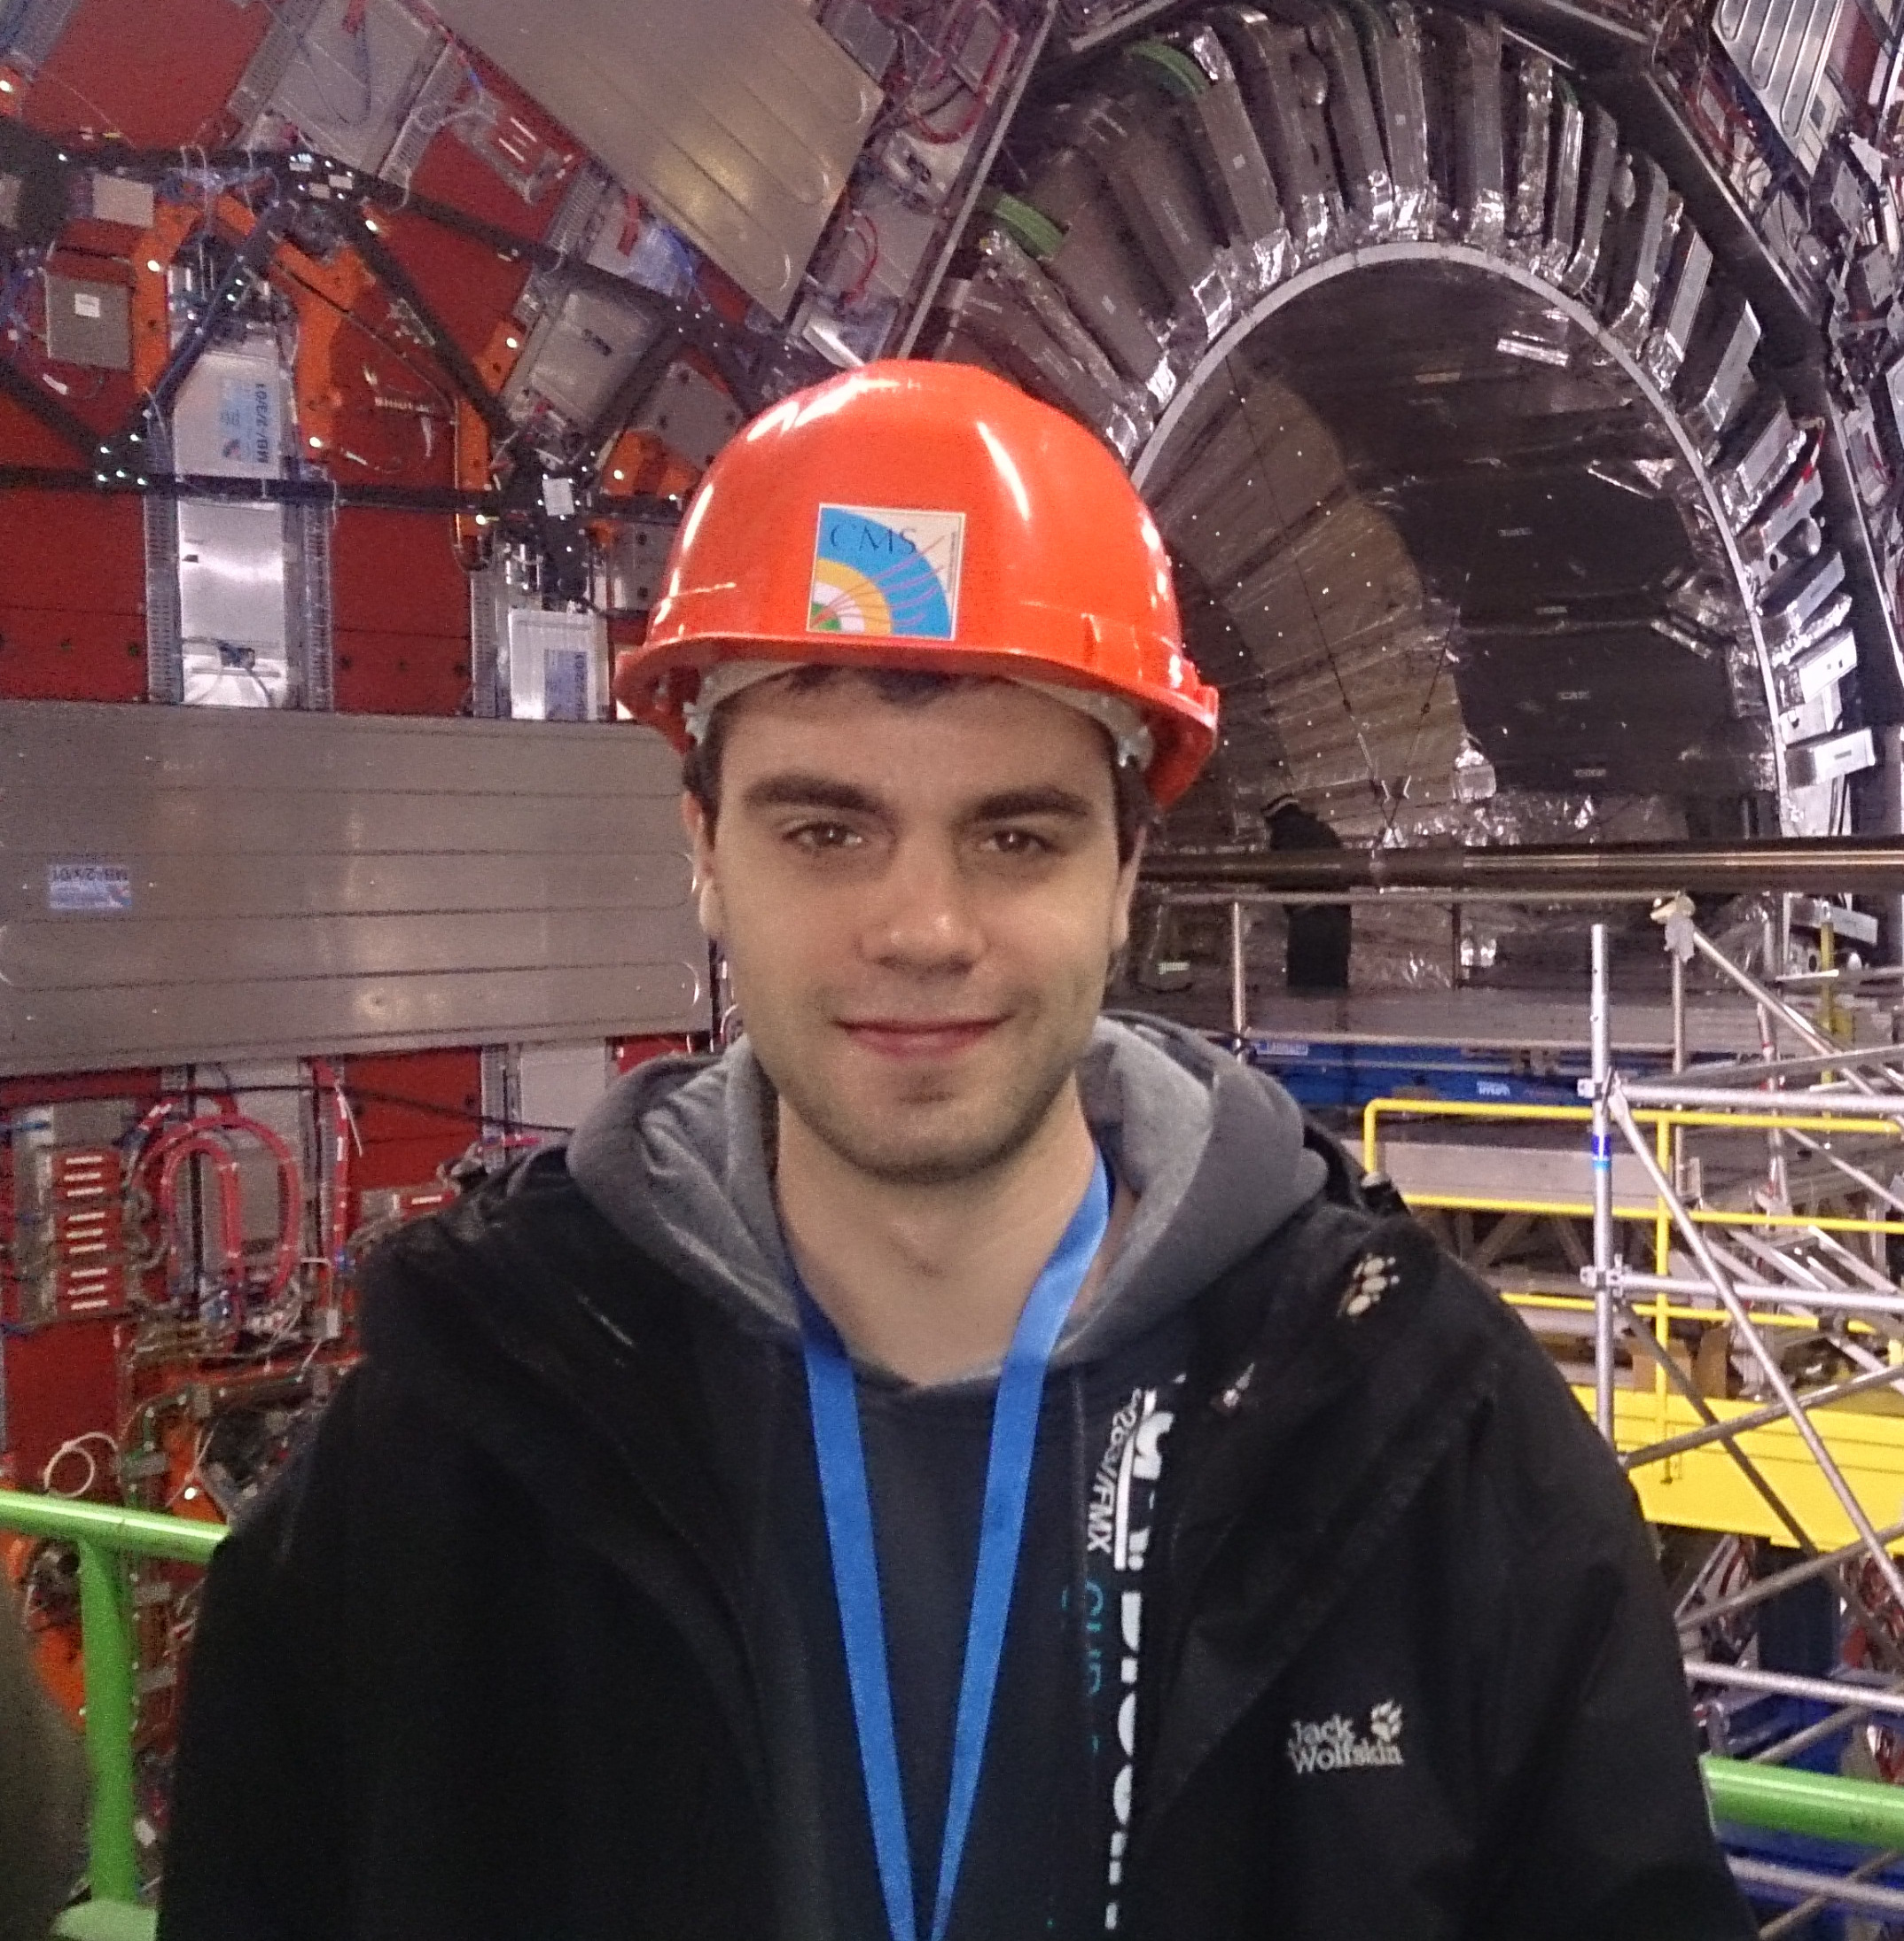
\includegraphics[width=6em,height=6em]{HackathonSlides/Pictures/DSC_0762.JPG}
\caption{Jan-Lukas Wynen}
\end{figure}
\end{column}
\end{columns}
\begin{columns}
\begin{column}{0.25\textwidth}
\begin{figure}
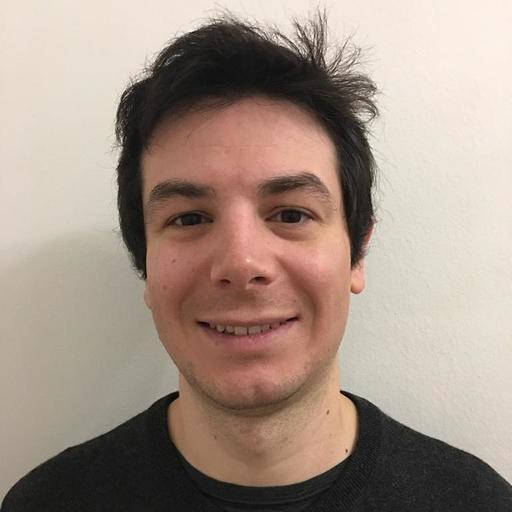
\includegraphics[width=6em,height=6em]{HackathonSlides/Pictures/Gonzalo.jpg}
\vspace*{-2em}
\caption{Gonzalo Brito}
\end{figure}
\end{column}
\begin{column}{0.25\textwidth}
\begin{figure}
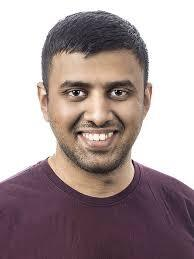
\includegraphics[width=5em,height=6em]{HackathonSlides/Pictures/jayesh.jpg}
\vspace*{-2em}
\caption{Jayesh Badwaik}
\end{figure}
\end{column}
\begin{column}{0.5\textwidth}

\end{column}
\end{columns}
\end{frame}
\setbeamertemplate{caption}[default]

\begin{frame}{Progress}
\begin{itemize}
\item \textbf{Problem} Singularity server crash (too little memory)\\
      Trying workaround without container\\[2ex]
\item Built locally with NVTX tracing:
\begin{itemize}
\item C++: working
\item Python: under construction
\end{itemize}
\end{itemize}
\end{frame}

\begin{frame}{Profile of existing Code}
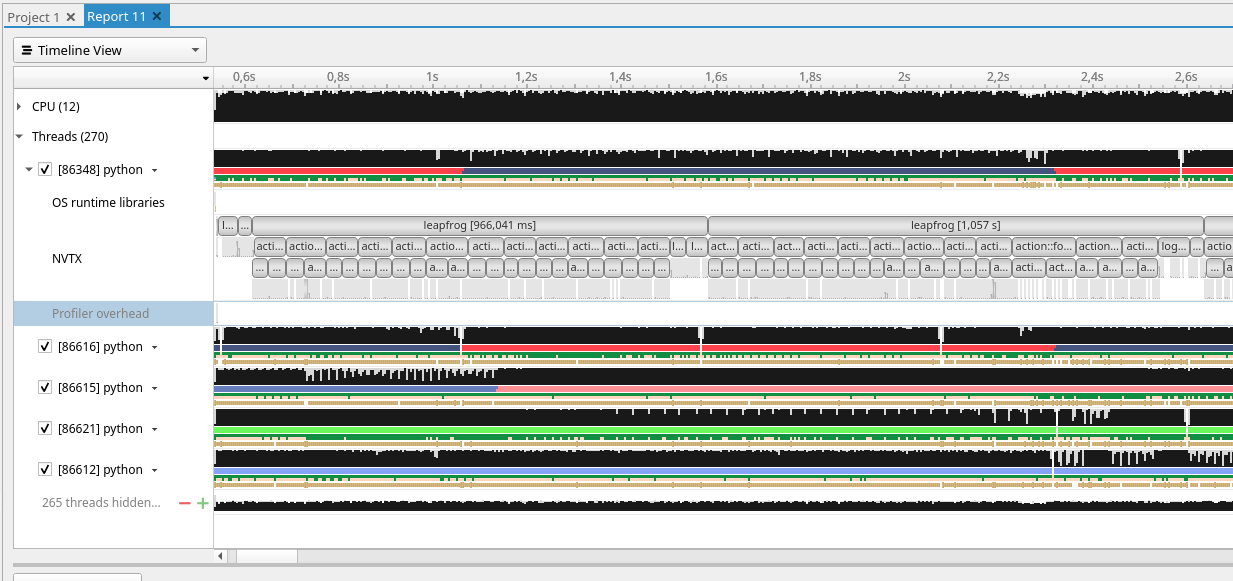
\includegraphics[width=\framewidth]{HackathonSlides/Pictures/profile_timeline_cpu.png}
\end{frame}

\begin{frame}{Next steps}
\begin{itemize}
\item Compile with Nvidia HPC SDK to use managed memory
\item Translated first functions to GPU
\end{itemize}
\end{frame}

\end{document}
